%% Direttive TeXworks:
% !TeX root = ../../maltoni_niccolo_tesi.tex
% !TEX encoding = UTF-8 Unicode
% !TEX program = arara
% !TEX TS-program = arara
% !TeX spellcheck = it-IT

\chapter{Contributo}\label{ch:contributo}
    In questo capitolo verrà analizzato il contributo fornito al progetto, elencando i requisiti necessari e analizzando il processo di soddisfazione degli stessi.

    L'obiettivo principale è quello di integrare una nuova interfaccia per la simulazione, al fine di semplificare l'adozione del simulatore da parte di utenti inesperti.

    \section{Analisi dei requisiti}\label{sec:analisi}
        Lo studio del lavoro illustrato in questa tesi ha inizio con l'analisi dei requisiti dell'interfaccia utente, ossia cosa l'applicazione deve mostrare a schermo.

        Questa sezione si occuperà di enunciare i requisiti funzionali e non funzionali individuati.

        \subsection{Requisiti funzionali}\label{subsec:funzionali}
            I requisiti funzionali descrivono il comportamento che il sistema deve avere:
            descrivono le funzionalità del sistema software, in termini di servizi che il sistema software deve fornire, di come il sistema software reagisce a specifici tipi di input e di come si comporta in situazioni particolari.

            \subsubsection{Rappresentazione dell'ambiente di simulazione}\label{subsubsec:seeEnv}
                Essendo la componente grafica da reimplementare quella legata alla simulazione in esecuzione, requisito fondamentale è che la GUI possa rappresentare l'ambiente con le maggiori possibilità di dettaglio possibile.

                Di conseguenza, deve essere presente uno spazio disegnabile in cui si possa avere una rappresentazione grafica di quanto accade, ma anche contatori che mostrino l'avanzamento della simulazione in termini di tempo (secondi) trascorso e passaggi (\engEmph{step}) effettuati.

            \subsubsection{Gestione degli effetti}\label{subusubsec:manageEffects}
                La nuova interfaccia deve rendere possibile all'utente di poter aggiungere nuovi effetti allo \engEmph{stack} di rappresentazione e modificarne le proprietà a tempo di esecuzione.

                Inoltre, attraverso la GUI l'utente deve poter salvare la pila di effetti presente in quel momento e caricarla in un secondo momento, mantenendo tutte le proprietà definite manualmente.

                Infine, deve essere possibile nascondere singoli effetti o gruppi di essi senza rimuoverli dallo \engEmph{stack}.

            \subsubsection{Serializzazione \engEmph{Human-readable}}
                In riferimento al punto precedente, deve essere possibile serializzare gli effetti in formato testo, in modo tale che file compatibili possano essere creati e/o modificati manualmente in modo semplice, senza coinvolgere necessariamente l'interfaccia di Alchemist.

            \subsubsection{Effetti standard per nodi e collegamenti}\label{subusubsec:defaultEffects}
                Devono essere implementati effetti adibiti alla rappresentazione dei singoli nodi come punti e dei collegamenti tra i nodi di un vicinato.

                Questi effetti dovranno essere caricati automaticamente al lancio dell'applicazione, salvo diversamente specificato.

            \subsubsection{Interazione con simulazione e ambiente rappresentato}\label{subsubsec:interazione}
                L'interfaccia deve mettere a disposizione dell'utente la capacità di interagire con la simulazione, potendo fermarla e riavviarla, interagire con i nodi e spostarsi tra essi.
                Deve essere possibile effettuare pan e zoom sull'ambiente rappresentato.

                Le possibilità di interazione non devono essere vincolate al puntatore del mouse, ma devono essere supportate anche le scorciatoie da tastiera.

            \subsubsection{Rappresentazione di ambienti con mappa}\label{subsubsec:mappa}
                Deve essere fornito il supporto alle mappe come sfondo degli ambienti nella rappresentazione di simulazioni che coinvolgano questo aspetto.

            \begin{figure}[htbp]
                \centering
                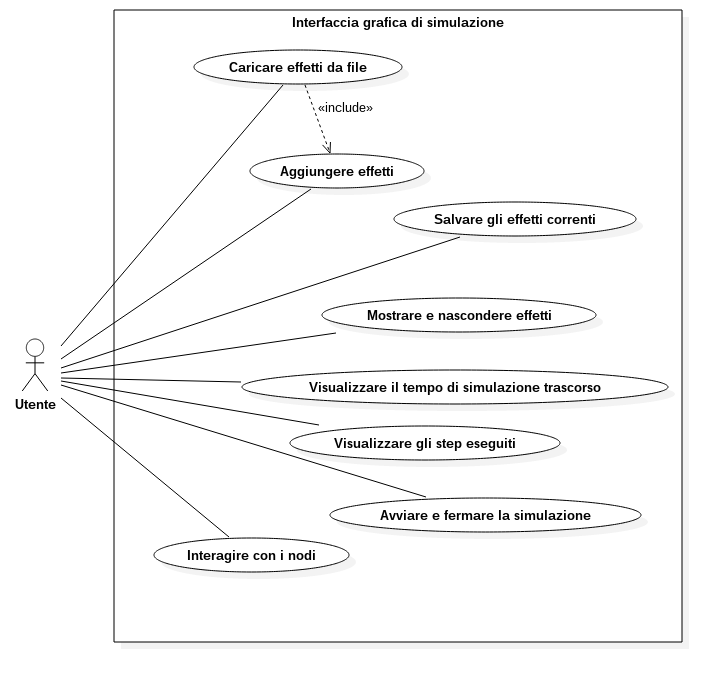
\includegraphics[scale=0.65]{img/useCase}
                \caption{Il diagramma UML rappresenta i casi d'uso principali dell'interfaccia}
                \label{fig:useCase}
            \end{figure}

        \subsection{Requisiti non funzionali}\label{subsec:nonFunzionali}
            I requisiti non funzionali descrivono le proprietà non comportamentali che il sistema deve possedere, come efficienza, affidabilità, sicurezza, performance, ma anche caratteristiche del processo di sviluppo e caratteristiche esterne.

            \subsubsection{JavaFX}\label{subsubsec:jfx}
                Come specificato nella \Cref{sec:motivi}, il processo di sviluppo deve coinvolgere la libreria JavaFX come framework per la costruzione dell'interfaccia.

            \subsubsection{Performance}\label{subsubsec:performance}
                L'interfaccia grafica deve quanto più possibile non gravare sulle prestazioni del motore di simulazione;
                in particolare, poiché JavaFX non è nativamente \engEmph{thread-safe}, è necessario gestire la concorrenza in modo oculato.

            \subsubsection{Supporto Hi-DPI}\label{subsubsec:hidpi}
                L'interfaccia non deve perdere di usabilità e qualità di rappresentazione su alcun tipo di schermo, indipendentemente dalla risoluzione e dalla densità di pixel.
                Per fare questo si devono quindi utilizzare quanto più possibile grandezze relative e sfruttare al meglio in tal senso le funzionalità offerte da JavaFX.

    \section{Stato dell'arte}\label{sec:ispirazione}
        Una volta chiariti i requisiti dell'interfaccia, il passo successivo riguarda la progettazione dell'interfaccia.

        Per poter disegnare dei mockup da utilizzare come bozzetti, sono state fatte ricerche in merito alle interfacce grafiche utilizzate da altri simulatori che costituivano lo stato dell'arte per quanto riguarda i software di simulazione, anche e soprattutto a scopo non strettamente scientifico.

        Infine, si è scelto tra i design moderni più comuni e apprezzati quale adottare al fine di ottenere un aspetto grafico a cui l'utente medio fosse già abituato e che potesse fornire un'esperienza di utilizzo più gradevole.

        \subsection{Simulatori a scopo videoludico}\label{subsec:videogame}
            Come già segnalato nelle sezioni precedenti, è importante che l'interfaccia grafica si presenti semplice e immediata anche per l'utente non avanzato.
            Di conseguenza, si è scelto di analizzare con più attenzione le GUI di simulatori sviluppati a scopo prettamente videoludico, in quanto più orientati all'immediatezza d'uso rispetto ai simulatori di concezione scientifica.

            Tra i videogiochi di simulazione più famosi, è stato interessante analizzare SimCity, il quale all'epoca del lancio fu molto apprezzato~\cite{friedman1995} appunto per il gameplay e l'interfaccia piuttosto innovativi, e i giochi della serie Universe Sandbox del team Giant Army.

            \subsubsection{SimCity}\label{subsubsec:simcity}
                La celebre serie di videogiochi di simulazione SimCity, ideata da Will Wright\footnote{Intervista per la rivista Wired, 1994:
                \url{https://www.wired.com/1994/01/wright}} tra gli anni `80 e gli anni `90 ispirandosi ai risultati della ricerca contenuta nel saggio di architettura \engEmph{A pattern language}~\cite{aPatternLanguage}, è sviluppata da Maxis e distribuita da Electronics Arts ed è tutt'ora considerata una delle più innovative per quanto riguarda la storia dei videogiochi di simulazione.

                \begin{figure}[htbp]
                    \centering
                    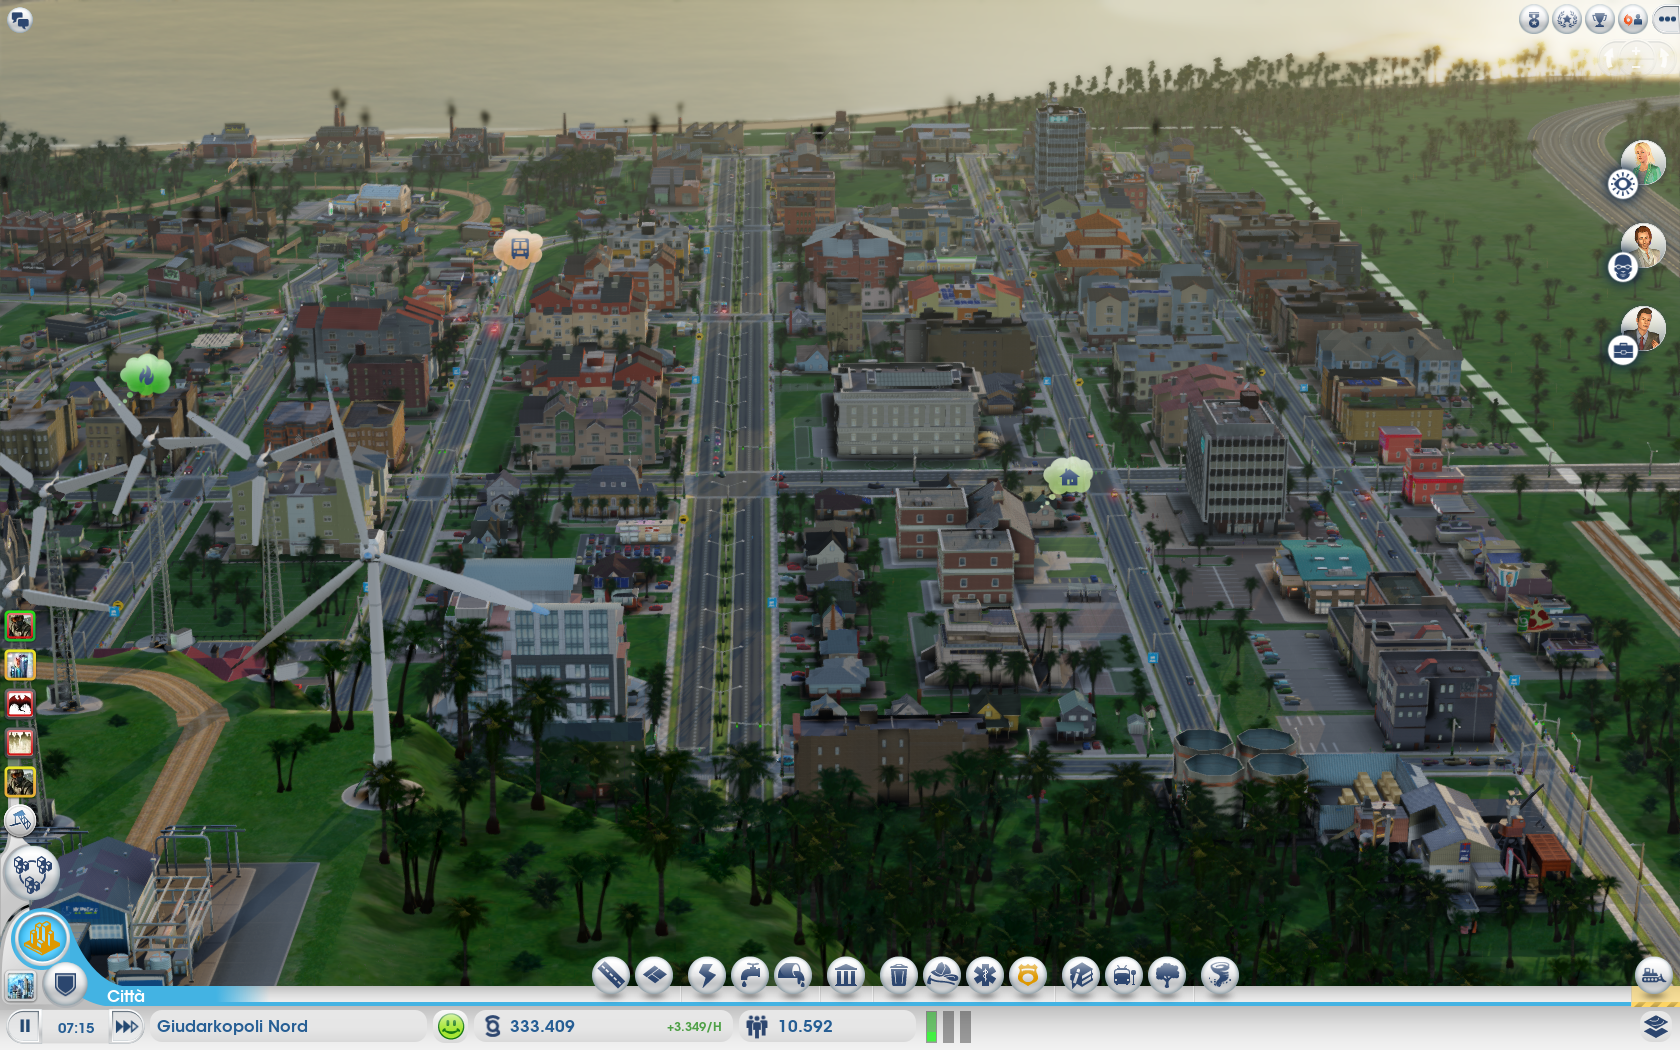
\includegraphics[scale=0.24]{img/SimCity}
                    \caption{Interfaccia grafica di SimCity (2013), sviluppato da Maxis e distribuito da EA}
                    \label{fig:simcity}
                \end{figure}

            \subsubsection{Universe Sandbox}\label{subsubsec:universesandbox}
                Altra serie di videogiochi simulativi analizzata è Universe Sandbox.
                Dopo oltre 15 anni di sviluppo\footnote{Analisi di Alex Cox per il blog TechCrunch, 2008:
                \url{http://www.techradar.com/news/software/computing/how-one-man-created-his-own-universe-470870}}, il primo capitolo è stato rilasciato dallo sviluppatore e artista Dan Dixon nel 2008.
                Il responso positivo lo ha portato a continuare lo sviluppo, tanto da fondare la compagnia Giant Army\footnote{attualmente composta da Dan Dixon, Christian Herold, Georg Steinröhder, Thomas Grønneløv, Eric Hilton, Naomi Goldenson e Chad Jenkins}, che ha rilasciato nel 2015 la seconda iterazione della saga, Universe Sandbox 2.

                Per il design dell'interfaccia, è stato proprio il secondo capitolo a fungere da maggior fonte d'ispirazione.
                Essa va a riprendere la classica interfaccia utilizzata da videogiochi simulativi come il già citato SimCity, ma andando a rimuovere buona parte degli ornamenti grafici tipici delle GUI a scopo videoludico, andando a preferire uno stile molto più pulito e semplificato;
                il sistema di interazione a sviluppo verticale e a popup (\Cref{fig:simcity}) viene sostituito con uno sviluppo orizzontale di pannelli (definito \emph{Modello multi-paned}~\cite{multipanedmodel}) che vanno a raccogliere tutte le impostazioni e i parametri (\Cref{fig:universesandboxpanels}).

                La simulazione viene rappresentata sullo sfondo, come in SimCity, ma con effetti di trasparenza non presenti nel gioco di EA.

                \begin{figure}[htbp]
                    \centering
                    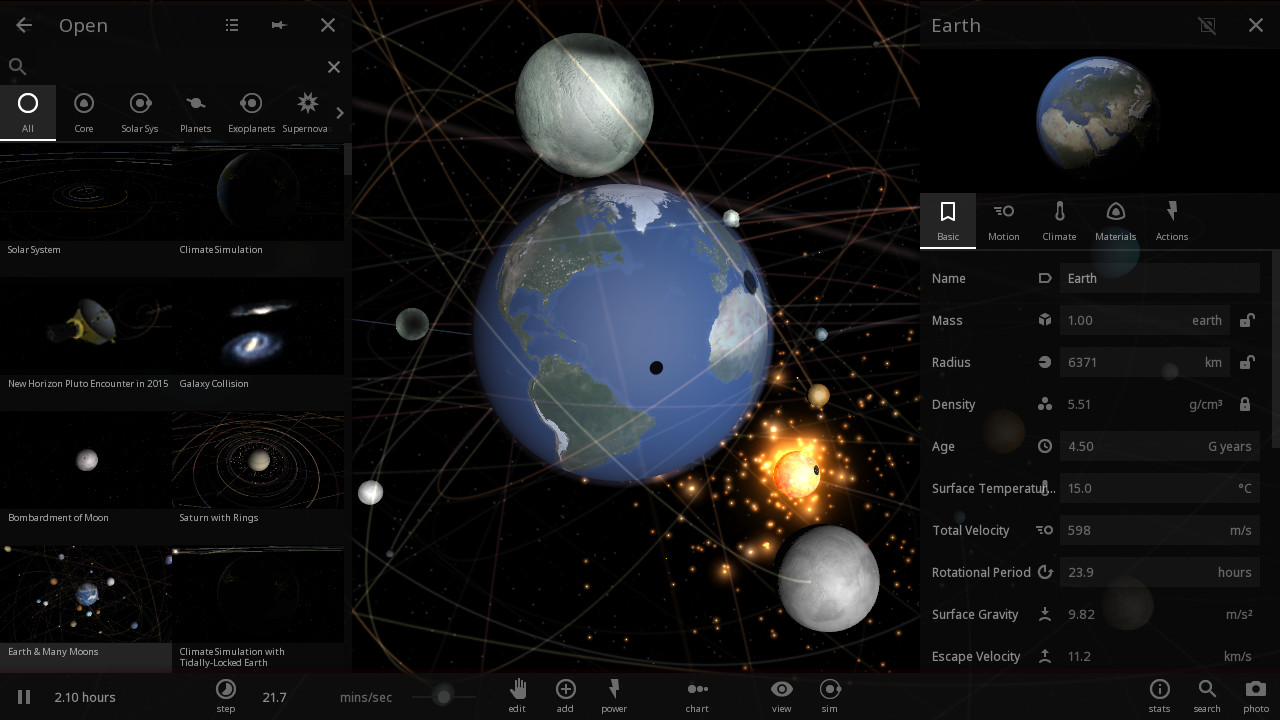
\includegraphics[scale=0.32]{img/universesandboxpanels}
                    \caption{Rappresentazione dell'interfaccia di Universe Sandbox 2 (2015), sviluppato e distribuito da Giant Army}
                    \label{fig:universesandboxpanels}
                \end{figure}

        \subsection{Material Design}\label{subsec:material}
            Uno dei maggiori motivi che hanno portato l'interfaccia grafica di Alchemist a necessitare di un rinnovamento è stata l'intenzione di semplificarla all'occhio dell'utente non esperto, fornendo un'esperienza completa e gradevole.
            Era dunque necessario scegliere uno stile grafico familiare, moderno e facilmente adattabile a quella che sarebbe essere la nuova interfaccia che si stava progettando.

            Prendendo come base l'interfaccia di Universe Sandbox 2 illustrata nella \Cref{subsubsec:universesandbox}, è possibile notare che il design di base sia estremamente ``\engEmph{flat}'';
            si è deciso di valutare i possibili design a cui adeguare la UX che si aveva intenzione di progettare.

            La scelta è infine ricaduta sul Material Design sviluppato da Google:
            dal suo annuncio nel giugno del 2014 al Google I/O 2014 Keynote esso è stato almeno parzialmente adottato in molte applicazioni web, mobile e desktop e ben si si presta all'implementazione di un'interfaccia semplice e minimale.

            Si è deciso di utilizzare le icone\footnote{\url{https://material.io/icons/}} e le direttive in merito a dimensioni e palette di colore\footnote{\url{https://material.io/color/}} fornite da Google.

    \section{Design dell'interfaccia}\label{sec:design}
        Una volta chiariti i requisiti e le possibili fonti di ispirazione per la struttura della GUI da realizzare, sono stati disegnati dei mockup che potessero rappresentare una linea guida per l'implementazione concreta dell'interfaccia.

        \begin{figure}[htbp]
            \centering
            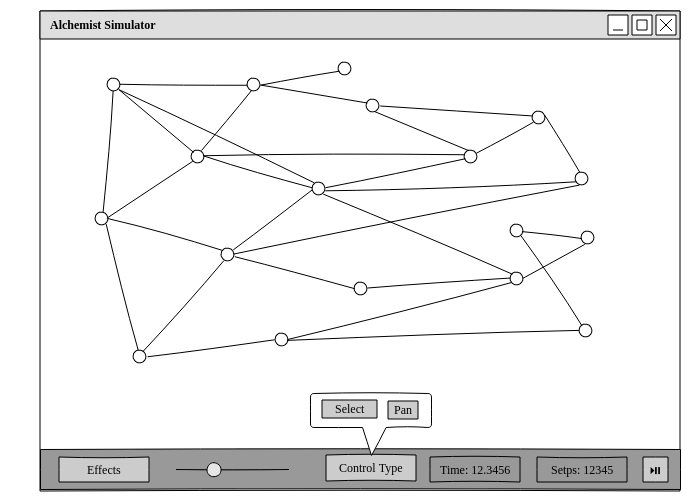
\includegraphics[scale=0.5]{img/withNodes/main_window}
            \caption{Mockup dell'interfaccia principale}
            \label{fig:mock:mainWindow}
        \end{figure}

        Come è possibile vedere dalla \Cref{fig:mock:mainWindow}, si è scelto di adottare un'interfaccia composta da uno spazio disegnabile centrale, al quale viene sovrapposta nella parte inferiore una barra contenente dei controlli che permettono un'interazione semplice e diretta con le funzionalità di base:

        \begin{description}
            \item [Play/Pausa]
                Partendo da destra, è presente un bottone che permette di avviare e mettere in pausa la simulazione.

                Esso funge anche da indicatore per lo stato attuale della simulazione:
                qualora essa venga avviata o fermata da terminale o tramite una scorciatoia da tastiera, l'icona rappresentata sul bottone viene aggiornata per adeguarsi al nuovo stato.

            \item[Avanzamento in termini di tempo e step]
                Continuando verso sinistra, si trovano spazi dedicati al numero di secondi di simulazione rappresentati e di step effettuati;
                essi vengono aggiornati durante tutto l'avanzamento del motore di simulazione.

            \item[Gestione del sistema di controllo]
                Poiché l'interazione tramite mouse deve permettere sia di spostarsi nell'ambiente che selezionare i nodi e interagirvi, è presente un bottone che apre un pannello che permette di scegliere tra spostamento (\engEmph{pan}) e selezione.

            \item[Gestione della velocità]
                Una barra a scorrimento permette di regolare la velocità di rappresentazione della simulazione.

            \item[Gestione degli effetti]
                Un bottone sul lato sinistro della barra permette di aprire un pannello sul medesimo lato della finestra per poter controllare gli effetti con i quali rappresentare cosa sta avvenendo nella simulazione.

                % Nelle \Crefrange{fig:mock:groups}{fig:mock:properties} è possibile osservare i diversi livelli del drawer laterale degli effetti.
                Nella \Cref{fig:mock:allEffects} è possibile osservare i diversi livelli del drawer laterale degli effetti.

                \begin{figure}[htbp]
                    \centering%
                    \subfigure[%
                        Vista dei singoli gruppi di effetti che compongono lo \engEmph{stack}%
                        \label{fig:mock:groups}
                    ]{%
                        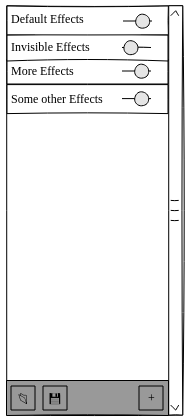
\includegraphics[scale=0.5]{img/cropped/effectgroups_bar_open}
                    }%
                    \qquad{\LARGE$\Rightarrow$}\qquad
                    \subfigure[%
                        Vista dei singoli effetti di un gruppo%
                        \label{fig:mock:effects}%
                    ]{%
                        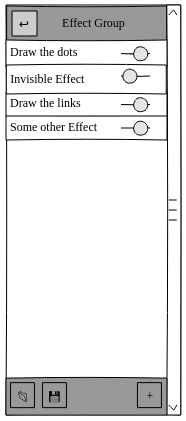
\includegraphics[scale=0.5]{img/cropped/effects_bar_open}
                    }%
                    \qquad{\LARGE$\Rightarrow$}\qquad
                    \subfigure[%
                        Vista delle proprietà di un effetto%
                        \label{fig:mock:properties}%
                    ]{%
                        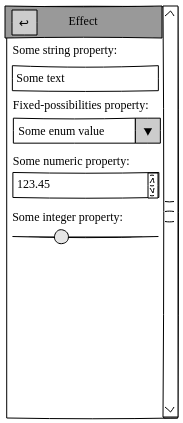
\includegraphics[scale=0.5]{img/cropped/effect_properties_open}
                    }
                    \caption{Mockup del pannello laterale degli effetti nei diversi livelli\label{fig:mock:allEffects}}
                \end{figure}

                % TODO sistema altezza frecce
        \end{description}

    \section{Progettazione}\label{sec:progettazione}
        Terminata la realizzazione dei mockup, il passo successivo riguardava la progettazione della struttura del sistema software.
        Durante la progettazione, in molti casi ci si è serviti di pattern di progettazione specifici, secondo quanto definito dalla cosiddetta \engEmph{Gang of Four}\footnote{John Vlissides, Richard Helm, Ralph Johnson, Erich Gamma} nel loro celebre saggio~\cite{designPattern} del 1995.

        \subsection{L'architettura degli effetti}\label{subsec:effetti}
            \subsubsection{I singoli effetti e l'interfaccia \texttt{EffectFX}}\label{subsubsec:effectFX}
                La componente architetturale più complessa da progettare probabilmente è costituita dagli effetti.
                Infatti, concettualmente il nuovo archetipo di effetti (di cui è possibile vedere l'UML in~\Cref{fig:effectFX}% TODO % o con maggiori dettagli in~\Cref{app:effectfx}
                ) rappresenta un oggetto completamente diverso:

                \begin{itemize}
                    \item[--]\label{itm:eFXEnv}
                        esso non si relaziona più con il singolo nodo, del quale può considerare le proprietà, bensì con l'intero ambiente;
                        in questo modo, l'effetto agisce in blocco su un determinato tipo di entità allo stesso modo, garantendo una migliore uniformità di applicazione.

                    \item[--]\label{itm:eFXName}
                        esso ha un \emph{nome} che lo identifica dalle altre istanze della medesima classe;
                        questo permette all'utente di identificarlo con più semplicità e gestirlo in modo più naturale, soprattutto nel caso si trovi a gestire, attraverso l'interfaccia grafica, una moltitudine di effetti.

                    \item[--]\label{itm:eFXVis}
                        esso possiede un campo di \emph{visibilità} individuale, che permette di nasconderlo temporaneamente, aumentando le possibilità di rappresentazione anche per blocchi di effetti predefiniti.

                    \item[--]\label{itm:eFXobservable}
                        le proprietà peculiari di ciascun effetto sono pensate per implementare il pattern \engEmph{Observer}~\cite{observer}, permettendo di effettuare collegamenti con l'interfaccia in modo trasparente ed ottimizzato, in quanto gestito completamente dal framework di JavaFX.

                    \item[--]\label{itm:eFXjson}
                        infine, l'effetto viene serializzato in formato \engEmph{human-readable}, il quale facilita la creazione e la modifica anche al di fuori dell'interfaccia di Alchemist.

                        Si è scelto di utilizzare il formato JSON\footnote{\url{https://www.json.org/index.html}} (\engEmph{JavaScript Object Notation}~\cite{json}), un formato di testo per la serializzazione dei dati strutturati, basato sugli oggetti JavaScript, che risulta essere facile da leggere e scrivere per le persone e facile da generare e analizzarne la sintassi per le macchine;
                        è un formato di testo indipendente dal linguaggio di programmazione, ma utilizza convenzioni riconosciute dalla maggior parte dei programmatori di linguaggi.

                \end{itemize}

                \begin{figure}[htbp]
                    \centering
                    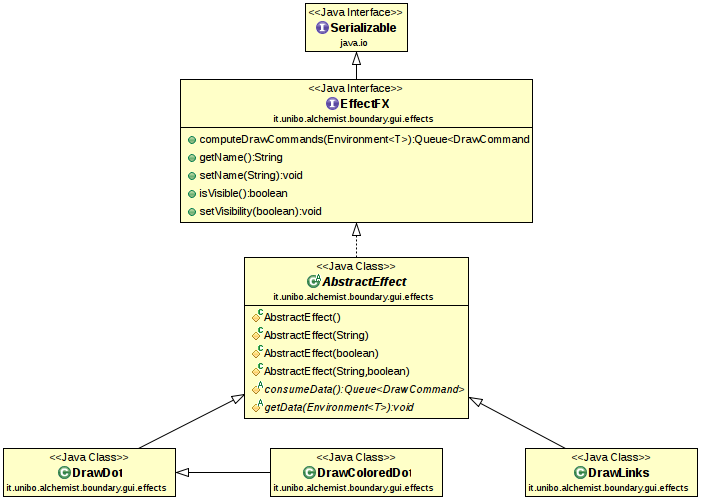
\includegraphics[scale=0.5]{img/EffectFXUMLsimple}
                    \caption{%
                        Diagramma UML delle classi che modellano la nuova struttura di effetti%; TODO
                        % TODO maggiori dettagli in \Cref{app:effectfx} %
                    }
                    \label{fig:effectFX}
                \end{figure}

                Come rappresentato graficamente nel diagramma UML in \Cref{fig:effectFX}, un effetto viene concretizzato secondo il pattern \engEmph{Template Method}~\cite{templateMethod}:
                la struttura di funzionamento di base viene parzialmente definita da una classe astratta che implementa il metodo principale dell'interfaccia effetto, \texttt{computeDrawCommands()}, come metodo template, il quale chiama i due metodi astratti \texttt{getData()} e \texttt{consumeData()} per adempiere al proprio compito.
                La suddivisione permette a ciascun effetto concreto di separare le procedure che coinvolgono l'interrogazione del modello da quelle che portano alla costruzione della coda di comandi per effettuare la rappresentazione grafica.

            \subsubsection{I gruppi di effetti e l'interfaccia \texttt{EffectGroup}}\label{subsubsec:effectGroup}
                L'esigenza di permettere all'utente di poter realizzare rappresentazioni complesse con numerosi effetti ha portato alla definizione di una classe collezione specifica:
                \begin{itemize}
                    \item[--]\label{itm:eFXgIterator}
                        la classe, secondo il contratto classico definito dall'interfaccia \texttt{Collection} di Java, è pensata per essere iterabile~\cite{iterator} e per permettere l'applicazione in blocco degli effetti che la compongono;

                    \item[--]\label{itm:eFXgName}
                        anche il gruppo di effetti è definito da un nome che lo distingue dagli altri, permettendo all'utente di distinguerli in modo più immediato;

                    \item[--]\label{itm:eFXgVis}
                        altra proprietà che accomuna la collezione con gli oggetti che è stata pensata per contenere è la visibilità:
                        essa permette di mostrare e nascondere in blocco tutti i suoi effetti senza andare a modificare la visibilità di ciascuno degli effetti;
                        l'interfaccia consente comunque di agire anche singolarmente sulla visibilità dei singoli nodi.
                \end{itemize}

            \subsubsection{Caricamento, salvataggio e modifica di gruppi di effetti}\label{subsubsec:serializzazione}
                Come detto~\vpageref{itm:eFXjson}, il salvataggio e il caricamento degli effetti avvengono tramite file JSON.
                Si è deciso di modellare una \engEmph{stateless utility class} che si comportasse da intermediario con la libreria utilizzata per la serializzazione, comportandosi secondo il pattern strutturale di tipo \engEmph{Façade}~\cite{designPattern}.
                È possibile vedere la rappresentazione UML in \Cref{fig:serial}.

                \begin{figure}[htbp]
                    \centering
                    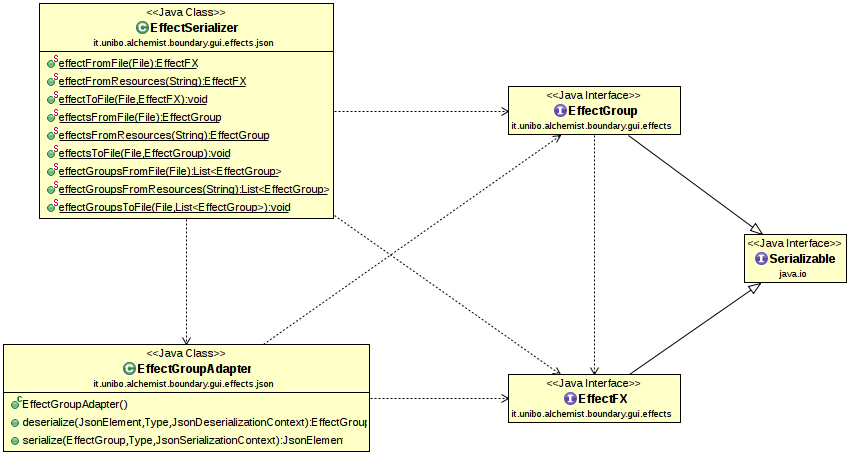
\includegraphics[scale=0.45]{img/EffectSerializationUML}
                    \caption{Diagramma UML delle classi che modellano la logica di serializzazione degli effetti tramite \engEmph{Façade stateless}}
                    \label{fig:serial}
                \end{figure}

        \subsection{La struttura dei drawer e le proprietà osservabili}\label{subsec:drawer}
            Una volta realizzato il mockup illustrato nella \Cref{sec:design}, l'attenzione si è spostata su progettarne la struttura a livello software.
            Trascurando i dettagli implementativi prettamente legati all'implementazione grafica, di cui si parla nella \Cref{sec:dettagli}, è stato importante progettare la gestione degli eventi di modifica di proprietà di effetti e gruppi.
            Come detto nella \Cref{itm:eFXobservable}, si è deciso di fare ampio uso del pattern \engEmph{Observer}, ciascun effetto è progettato per implementare proprietà osservabili%(UML in \Cref{fig:props})
            , che possono implementare ascoltatori di eventi dedicati in modo semplice, potendosi avvalere delle API messe a disposizione dal framework JavaFX.

            % \begin{figure}[htbp]
            %     \centering
            %     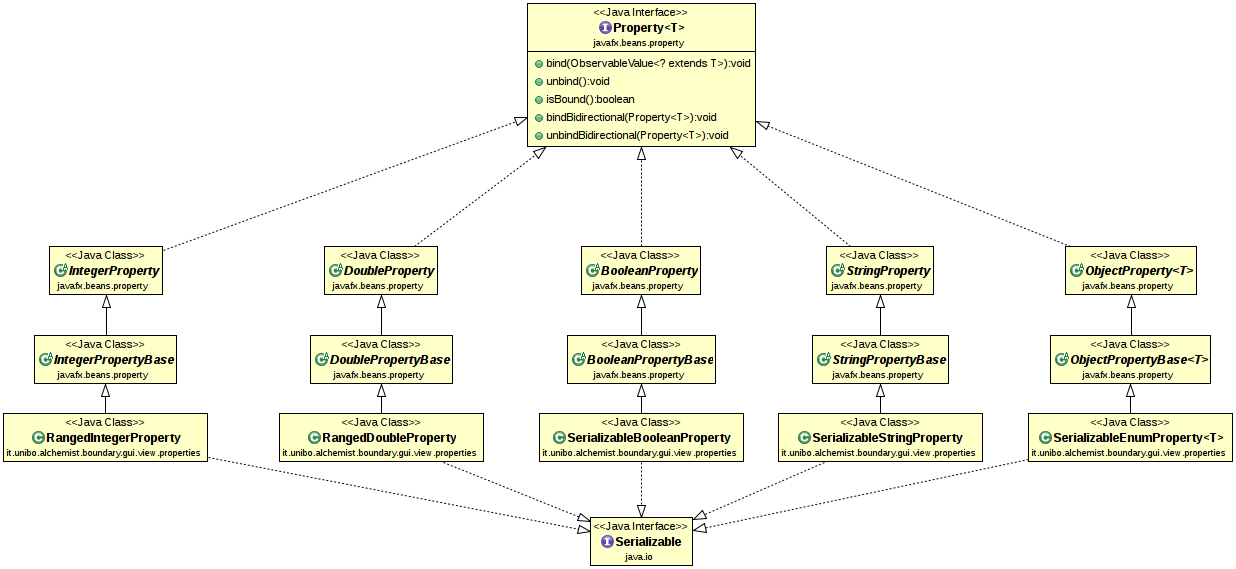
\includegraphics[scale=0.4]{img/PropertiesUMLsimple}
            %     \caption{Diagramma UML delle classi che modellano la logica delle proprietà serializzabili e osservabili implementate}
            %     \label{fig:props}
            % \end{figure}

        \subsection{Nodi grafici come monitor per la simulazione}
            Il canvas in cui vengono rappresentati gli effetti, il bottone che controlla l'avvio della simulazione e le etichette che mostrano il progresso della simulazione in termini di tempo e step sono indubbiamente nodi grafici;
            in fase di progettazione, si è scelto però di modellarli anche come monitor per il motore della simulazione, sfruttando ancora una volta il pattern \engEmph{Observer} per mettere in ascolto gli elementi della GUI legati alla simulazione stessa al fine di ricevere comunicazione di doversi aggiornare ad ogni step eseguito che li riguardi.

        \subsection{Costruzione e avvio dell'interfaccia}\label{subsec:avvio}
            L'interfaccia classica gestiva l'avvio della GUI per la simulazione in tempo reale, costruendo l'interfaccia con componenti Swing specifici assemblati in base ai parametri richiesti.

            La nuova interfaccia grafica è progettata conservando l'impiego di pattern \engEmph{Builder}, presentando un oggetto adibito all'interpretazione dei parametri e alla semplificazione del processo di costruzione.
            Si differenzia però per l'assenza di frammentazione della struttura:
            essa è modellata come un'unica applicazione JavaFX, con un layout predefinito, e il builder si occupa di modificare il comportamento e il tipo di canvas per adattarlo alla simulazione, oltre a caricare gli effetti e la simulazione stessa, ma non influenza l'aspetto della UI.

    \section{Dettagli implementativi}\label{sec:dettagli}

        \subsection{La barra inferiore}\label{subsec:barra}
            La barra inferiore (\Cref{fig:newBar}) è stata trasposta quasi perfettamente dal mockup al codice:
            si è utilizzato la classe \texttt{javafx\dothyp scene\dothyp control\dothyp ButtonBar} per modellare il layout della barra, mentre sono state impiegate le classi \texttt{JFXButton} e \texttt{JFXSlider} fornite nel package \texttt{com\dothyp jfoenix\dothyp controls} della libreria JFoenix per modellare i controlli mantenendoli sul prescelto stile del Material Design di Google.
            Il popup per la modifica del sistema di controllo è stato realizzato tramite la classe \texttt{org\dothyp controlsfx\dothyp control\dothyp PopOver} presente nella libreria ControlsFX.

            \begin{figure}[htbp]
                \centering
                
\includegraphics[scale=0.45]{img/NewBar}
                \caption{La barra inferiore concretamente realizzata}
                \label{fig:newBar}
            \end{figure}

            Gli effetti di colore e trasparenza sono stati implementati con diverse specifiche inserite nel foglio di stile CSS, inline nel documento FXML e attraverso i suddetti componenti.

        \subsection{Drawer, liste e celle}\label{subsec:drawerCelle}
            \begin{figure}[htbp]
                \centering%
                \subfigure[%
                    Vista dei singoli gruppi di effetti che compongono lo \engEmph{stack}%
                    \label{fig:impl:groups}
                ]{%
                    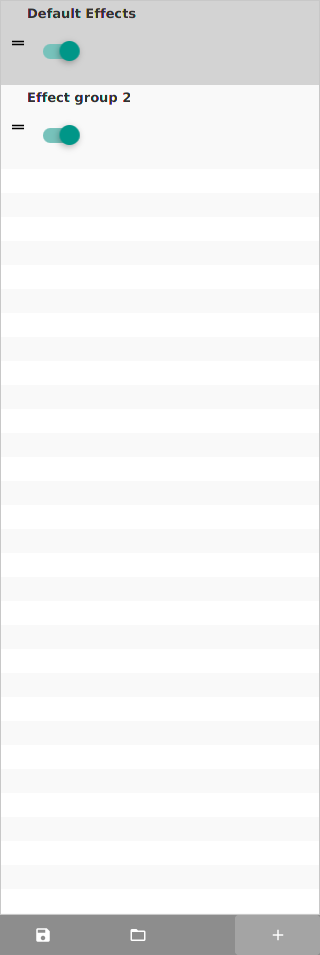
\includegraphics[scale=0.4]{img/cropped/effectgroups_bar_open_new}
                }%
                \qquad{\LARGE$\Rightarrow$}\qquad
                \subfigure[%
                    Vista dei singoli effetti di un gruppo%
                    \label{fig:impl:effects}%
                ]{%
                    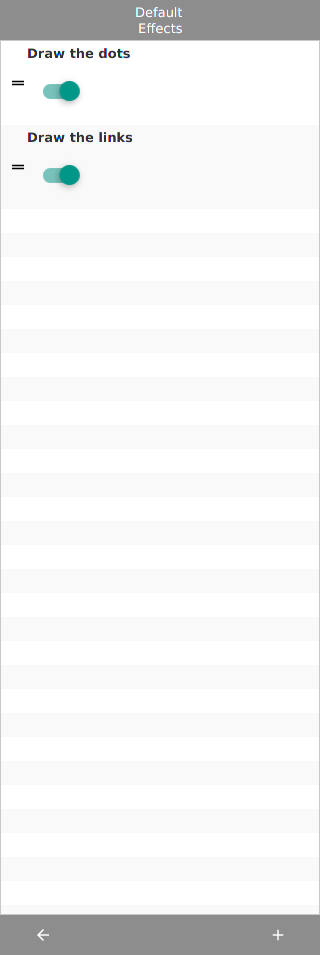
\includegraphics[scale=0.4]{img/cropped/effects_bar_open_new}
                }%
                \qquad{\LARGE$\Rightarrow$}\qquad
                \subfigure[%
                    Vista delle proprietà di un effetto%
                    \label{fig:impl:properties}%
                ]{%
                    
\includegraphics[scale=0.4]{img/cropped/effect_properties_open_new}
                }
                \caption{Vista del drawer laterale degli effetti nei diversi livelli\label{fig:impl:allEffects}}
            \end{figure}

            % TODO sistema altezza frecce

            L'impiego dei drawer, elemento tipico del Material Design, è stato possibile, ancora una volta, grazie alle classi \texttt{JFXDrawer} e \texttt{JFXDrawersStack} forniti da JFoenix.

            La struttura di un drawer è costituita dagli elementi seguenti:
            \begin{itemize}
                \item[--]
                    una opzionale barra superiore, che va a rappresentare il nome dell'elemento di cui si va a modificare il contenuto (ed è dunque assente nella vista di tutti i gruppi di effetti caricati);

                \item[--]
                    una barra inferiore, che fornisce possibili interazioni:
                    \begin{itemize}
                        \item[$\bullet$]
                            tornare al drawer precedente nello stack;
                            questa funzionalità è presente su ogni livello tranne il primo.
                        \item[$\bullet$]
                            aggiungere nuovi effetti o gruppi di effetti, andando a cercare tramite \engEmph{reflection} quelli presenti all'interno del classpath;
                            questa funzionalità è assente nel drawer che mostra le proprietà di uno specifico effetto.
                        \item[$\bullet$]
                            salvare e caricare gruppi di effetti da file;
                            questa funzionalità è disponibile solo nel primo drawer.
                    \end{itemize}

                \item[--]
                    la parte centrale del drawer, che può essere costituita da una \texttt{ListView} di \texttt{EffectFX} o di \texttt{EffectGroup}, o da una rappresentazione delle proprietà dell'effetto costruita a tempo di esecuzione sfruttando la \engEmph{reflection} per identificare quale nodo di controllo utilizzare.

                    Nel caso della lista, le celle sono state personalizzate per poter essere riordinate tramite \engEmph{drag'n'drop} e per permettere la modifica della visibilità tramite un \texttt{JFXToggleButton}.% e del nome tramite doppio click sulla relativa \texttt{Label}.
            \end{itemize}

            % TODO inserire immagini

        \subsection{Librerie esterne utilizzate}\label{subsec:lib}
            Per realizzare questa interfaccia grafica è stato necessario utilizzare delle librerie esterne che forniscono ulteriori funzionalità.
            Le librerie esterne utilizzate sono le seguenti.

            \subsubsection{ControlsFX}\label{subsubsec:controlsfx}
                Controlsfx\footnote{\url{http://fxexperience.com/controlsfx}} è una libreria \engEmph{open-source} per JavaFX, fornita da FX Experience e sponsorizzata da Gluon, che mette a disposizione controlli per interfacce di alta qualità e altri strumenti complementari a quelli distribuiti con JavaFX.
                È stata sviluppata per JavaFX 8 e successivi.

                È stata utilizzata per alcuni nodi ed elementi di layout.

            \subsubsection{JFoenix}\label{subsubsec:jfoenix}
                JFoenix\footnote{\url{http://www.jfoenix.com}} è una libreria \engEmph{open-source} per JavaFX che implementa il Google Material Design utilizzando i componenti Java.

                È stata impiegata per implementare per buona parte dei componenti della GUI in quanto già configurata per integrarsi in una UI Material.

            \subsubsection{jIconFont}\label{subsubsec:jiconfont}
                jIconFont\footnote{\url{https://jiconfont.github.io}} fornisce API per rendere disponibili icone generate tramite i più comuni font di icone, quali \emph{Elusive}, \emph{Entypo}, \emph{Font Awesome}, \emph{Google Material Design Icons}, \emph{Open Iconic} e \emph{Typicons};
                è disponibile sia per Swing che per JavaFX.

                È stata usata nella sua versione per JavaFX con le icone del pacchetto \emph{Google Material Design Icons} per evitare di utilizzare numerosi file immagine e mantenere una perfetta scalabilità grafica anche a risoluzioni elevate.

            \subsubsection{Google Gson}\label{subsubsec:gson}
                Gson\footnote{\url{https://github.com/google/gson}} è una libreria Java \engEmph{open-source} sviluppata da Google adibita a convertire gli oggetti Java nella loro rappresentazione JSON e a convertire una stringa JSON nell'equivalente oggetto Java.

                È stata sfruttata per implementare la lettura e la scrittura del file JSON di salvataggio dei gruppi di effetti.

        \subsection{Strumenti utilizzati}\label{subsec:strum}
            \subsubsection{Qualità del codice e controllo del software}\label{subsubsec:codeQuality}
                Date le dimensioni di Alchemist, è necessario fare uso di strumenti che controllino la qualità del codice e diano la possibilità di testarlo in modo immediato.

                Gli strumenti di qualità del codice permettono di revisionare il codice in modo sistematico, così da evitare errori che a volte possono verificarsi, senza bisogno che il programma venga realmente eseguito:
                essi analizzano il codice sorgente per individuare potenziali bug o codice duplicato e per indicare i possibili miglioramenti e ottimizzazioni.

                Il progetto Alchemist utilizza i seguenti strumenti:

                \begin{description}
                    \item[FindBugs\label{itm:FindBugs}\footnotemark]\footnotetext{\url{http://findbugs.sourceforge.net}}
                        è un analizzatore di codice statico \engEmph{open-source} che rileva possibili bug all'interno del codice Java realizzato da Bill Pugh e David Hovemeyer e marchio registrato dall'Università del Maryland.

                        Classifica i potenziali errori in categorie, per dare un'idea migliore allo sviluppatore di quale potrebbe essere il loro impatto sul software;
                        opera direttamente sul bytecode di Java.

                    \item[Checkstyle\label{itm:Checkstyle}\footnotemark]\footnotetext{\url{http://checkstyle.sourceforge.net}}
                        è un analizzatore di codice statico \engEmph{open-source} per diversi linguaggi di programmazione che verifica che il codice scritto aderisca a un determinato stile di codifica.

                        Esso effettua un controllo sulla presentazione e non sul contenuto, dunque non permette di assicurare la correttezza e la completezza del software.

                    \item[PMD\label{itm:PMD}\footnotemark]\footnotetext{\url{https://pmd.github.io}}
                        è uno strumento di analisi del codice sorgente statico per Java e altri linguaggi che prevede un set di regole, personalizzabile dallo sviluppatore, per definire quando una parte di esso è errata.

                        Generalmente, gli errori segnalati riguardano scelte implementative subottimali e imperfezioni nel codice, che non inficiano direttamente il funzionamento del programma ma per la maggior parte il livello del sorgente.

                        Componente importante è il \emph{Copy/Paste Detector} (CPD) che utilizza l'algoritmo di Rabin–Karp per la ricerca delle stringhe~\cite{RabinKarp}, che permette di identificare codice duplicato con elevata precisione.
                \end{description}

            \subsubsection{Controllo di versione}\label{subsubsec:hosting}
                Il controllo di versione utilizzato per Alchemist è affidato al DVCS (\engEmph{Distributed Version Control System}) Git, utilizzato con flusso di lavoro di tipo \emph{Git flow}.

            \subsubsection{Automazione dello sviluppo e integrazione continua}\label{subsubsec:buildECI}
                Alchemist si avvale di Gradle per il processo di \engEmph{build automation} e di Travis CI per la fase di test in \engEmph{continuous integration} dopo l'aggiunta del codice al repository ufficiale su GitHub.

                \begin{description}
                    \item[Gradle\footnotemark]\footnotetext{\url{https://gradle.org}}
                        è un sistema per l'automazione dello sviluppo, nato per includere tutte le caratteristiche provenienti da Apache Ant, Maven e Ivy attraverso la definizione di \engEmph{buildscript} in Groovy.
                        Pensato per i linguaggi che compilano per JVM, questo sistema permette di avere una gestione controllata delle dipendenze (\engEmph{dependency management}), le quali vengono scaricate dai vari repository Maven durante la fase di compilazione.

                    \item[Travis CI\footnotemark]\footnotetext{\url{https://travis-ci.org}}
                        è un sistema di integrazione continua distribuito, utilizzato per la compilazione e il test di progetti caricati su repository GitHub;
                        è gratuito per progetti \engEmph{open-source}.

                        Il comportamento è definibile attraverso un file YAML;
                        Alchemist richiede di effettuare una procedura di \engEmph{building} completa con Gradle ad ogni commit su repository.
                \end{description}

            \subsubsection{Ambiente di sviluppo integrato}\label{subsubsec:IDE}
                Un IDE (\engEmph{Integrated Development Environment}), o ambiente di sviluppo integrato, è un software che aiuta i programmatori nello sviluppo del codice sorgente di un programma, mettendo a disposizione una serie di strumenti che permettono scrittura, compilazione o interpretazione, debug e analisi del codice da un unico ambiente, appunto, integrato.

                Durante lo sviluppo è stato utilizzato inizialmente Eclipse\footnote{\url{https://eclipse.org}} in versioni \textit{Neon.3} e \textit{Oxygen.1}, con l'integrazione dei plugin \emph{Gradle Buildship}, \emph{Xtext IDE}, \emph{Scala IDE}, \emph{e(fx)clipse}, \emph{FindBugs}, \emph{Checkstyle} e \emph{PMD}.

                Successivamente è stato utilizzato anche Jetbrains Intellij IDEA\footnote{\url{https://www.jetbrains.com/idea}} in versione \textit{Community 2017.2.6}, con l'integrazione dei plugin per il supporto a Scala e Xtend.

                In congiunzione ai due IDE per lo sviluppo del codice Java è stato utilizzato anche Gluon Scene Builder\footnote{\url{https://gluonhq.com/products/scene-builder}} per una prima definizione dei file FXML di layout.

        \section{Test e valutazione}\label{sec:test}
            \subsection{Unit testing e valutazione del codice}\label{subsec:junit}
                Durante lo sviluppo del codice si è prestata particolare attenzione alla qualità dello stesso: come detto \Cref{subsubsec:codeQuality}, sono stati utilizzati strumenti di analisi statica del codice (quali \emph{Checkstyle}, \emph{PMD} e \emph{FindBugs}) che potessero garantire una buona attinenza alle convenzioni e una riduzione delle possibilità di bug.

                Per garantire il corretto funzionamento delle funzionalità più cruciali non riguardanti strettamente collegate a elementi di interazione grafica, sono state create classi dedicate allo \engEmph{unit testing} attraverso la libreria JUnit\footnote{\url{http://junit.org}}, nella sua versione \href{http://junit.org/junit4/}{4.12}.

                In particolare, è stato testato a fondo il comportamento delle classi relative agli effetti, alla loro serializzazione e alle proprietà osservabili e serializzabili implementate: i risultati forniti dallo strumento di analisi della \engEmph{coverage} messo a disposizione da Intellij IDEA per i package \texttt{it\dothyp unibo\dothyp alchemist\dothyp boundary\dothyp gui\dothyp effects} e \texttt{it\dothyp unibo\dothyp alchemist\dothyp boundary\dothyp gui\dothyp view\dothyp properties}, ad esclusione delle classi precedenti annotate come deprecate, sono visibili in \Cref{fig:coverage}.

                \begin{figure}[htbp]
                    \centering
                    \frame{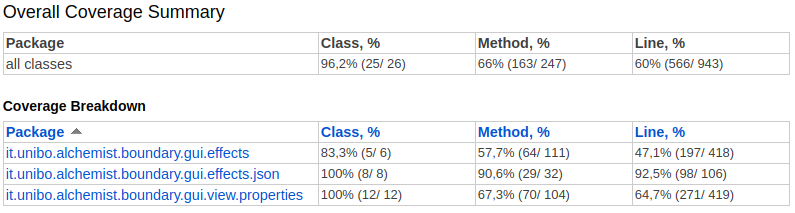
\includegraphics[scale=0.58]{img/filteredCoverage}}
                    \caption{Coverage per le classi relative agli effetti, alla loro serializzazione e alle proprietà osservabili e serializzabili implementate}
                    \label{fig:coverage}
                \end{figure}

            \subsection{Valutazione dell'interfaccia}\label{subsec:valutazione}
                L'interfaccia grafica risulta essere, per le funzionalità implementate, conforme ai requisiti concordati nella fase di analisi:

                \begin{itemize}
                  \item[--]
                      L'ambiente di simulazione è stato rinnovato, ed è in grado di renderizzare correttamente gli effetti applicati per una simulazione.
                      Inoltre, l'utente è in grado di visualizzare in tempo reale l'avanzamento della simulazione in termini di tempo e step tramite contatori dedicati.

                  \item[--]
                      La gestione degli effetti, accuratamente testata come specificato nella %\Cref{subsec:junit}
                      Sezione precedente, risulta immediata all'utilizzo, con bottoni dedicati al salvataggio e al caricamento dei file JSON (\Cref{fig:impl:groups}, barra inferiore) che aprono l'interfaccia fornita dal \engEmph{file manager} del sistema operativo per la scelta del file.

                      È possibile modificare l'ordine di effetti e gruppi di effetti nella pila con un semplice \engEmph{drag'n'drop} (\Cref{fig:simWithDnD}).

                      \begin{figure}[htbp]
                          \centering
                          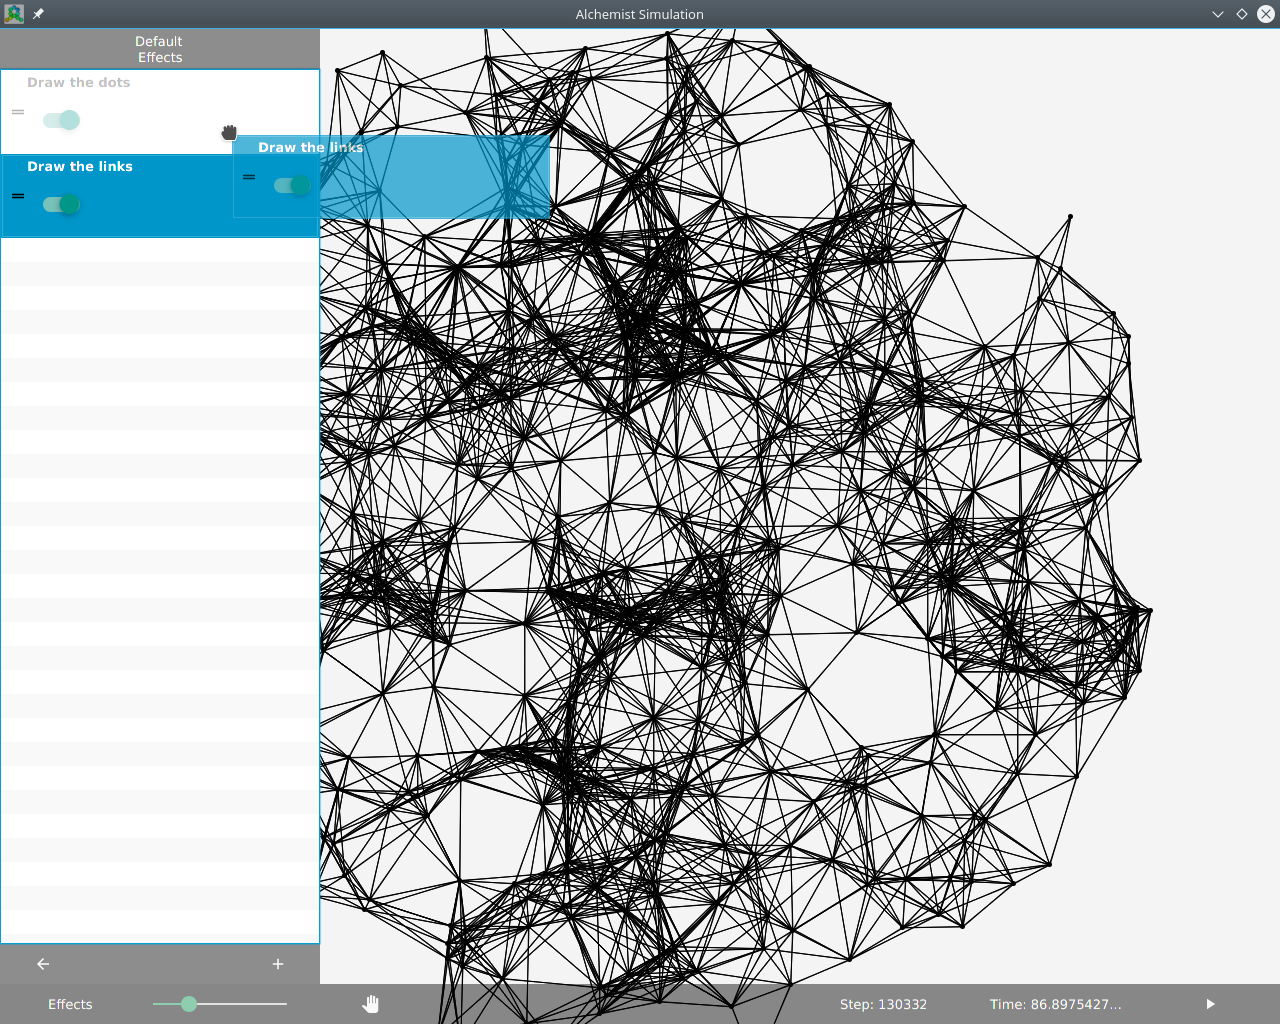
\includegraphics[scale=0.44]{img/withNodes/simWithDnD}
                          \caption{Gestione \engEmph{drag'n'drop} degli effetti}
                          \label{fig:simWithDnD}
                      \end{figure}

                  \item[--]
                      Sono stati realizzati effetti standard per la rappresentazione di nodi e collegamenti, che possono essere utilizzati da altri sviluppatori come punto di partenza per realizzare rappresentazioni più complesse e flessibili (\Cref{fig:simWithEff}).

                      \begin{figure}[htbp]
                          \centering
                          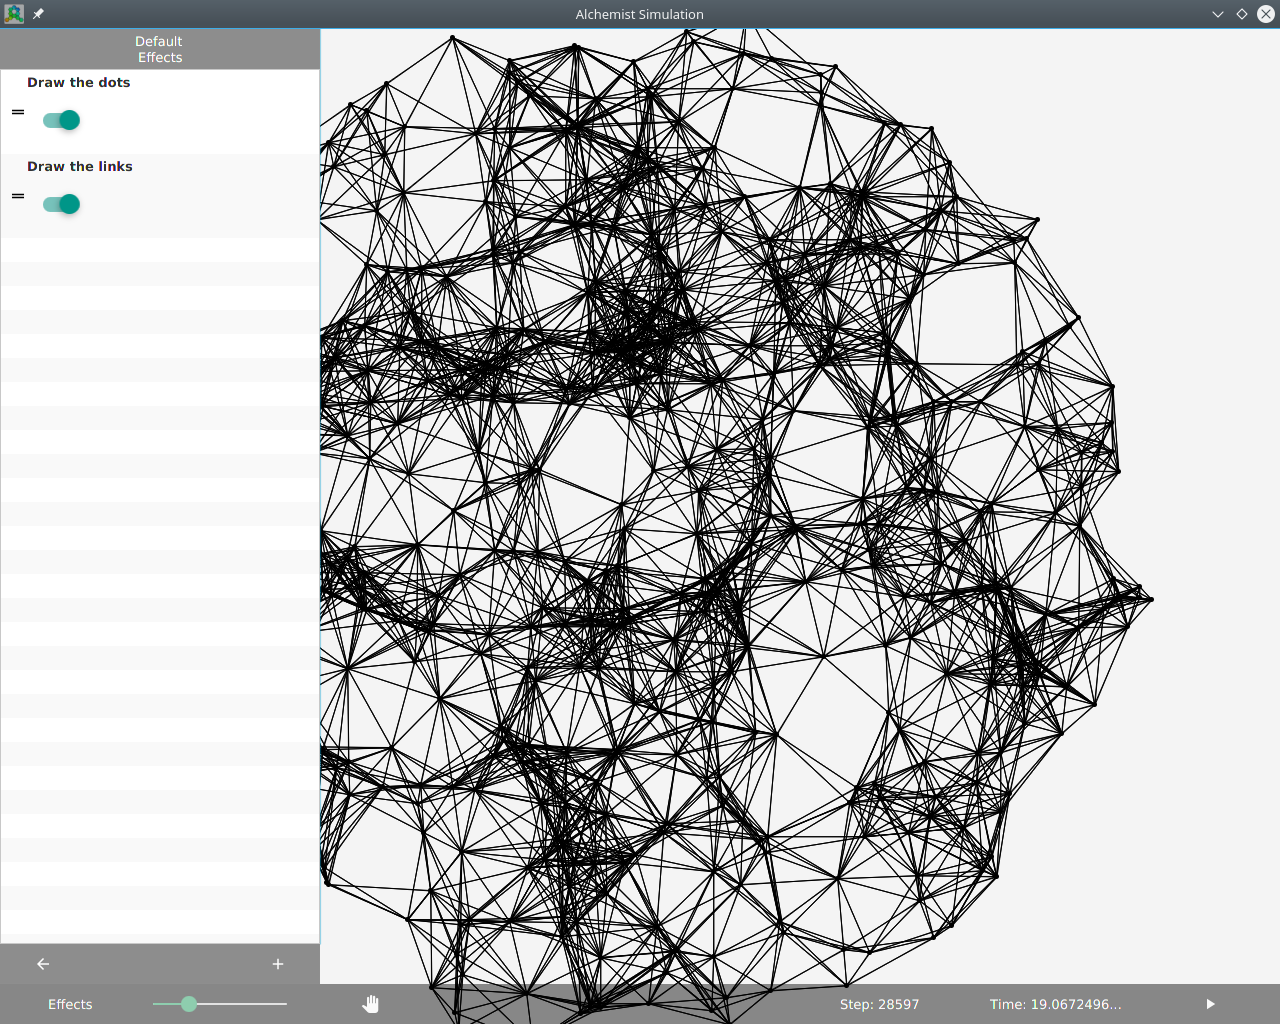
\includegraphics[scale=0.44]{img/withNodes/simWithEff}
                          \caption{Drawer laterale degli effetti aperto}
                          \label{fig:simWithEff}
                      \end{figure}

                  \item[--]
                      Le performance sono pienamente sufficienti: l'aumento di carico sulle risorse dovuto alla presenza di un'interfaccia grafica da renderizzare rientra in quanto preventivato nella fase di analisi.
                  \item[--]
                      L'interfaccia non utilizza valori di misura assoluti e scala perfettamente su diversi tipi di risoluzione e densità di pixel.
                  \item[--]
                      Le possibilità di interazione con l'ambiente di simulazione tramite mouse e tastiera sono presenti, ma limitate: è possibile controllarne il flusso di esecuzione sia tramite la pressione del tasto ``play/pausa'' che attraverso una scorciatoia da tastiera ed è possibile effettuare uno zoom nell'ambiente rappresentato tramite scroll.

                      Non è possibile, al momento, spostarsi nell'ambiente tramite \engEmph{drag'n'drop}.
                \end{itemize}

                \begin{figure}[htbp]
                    \centering
                    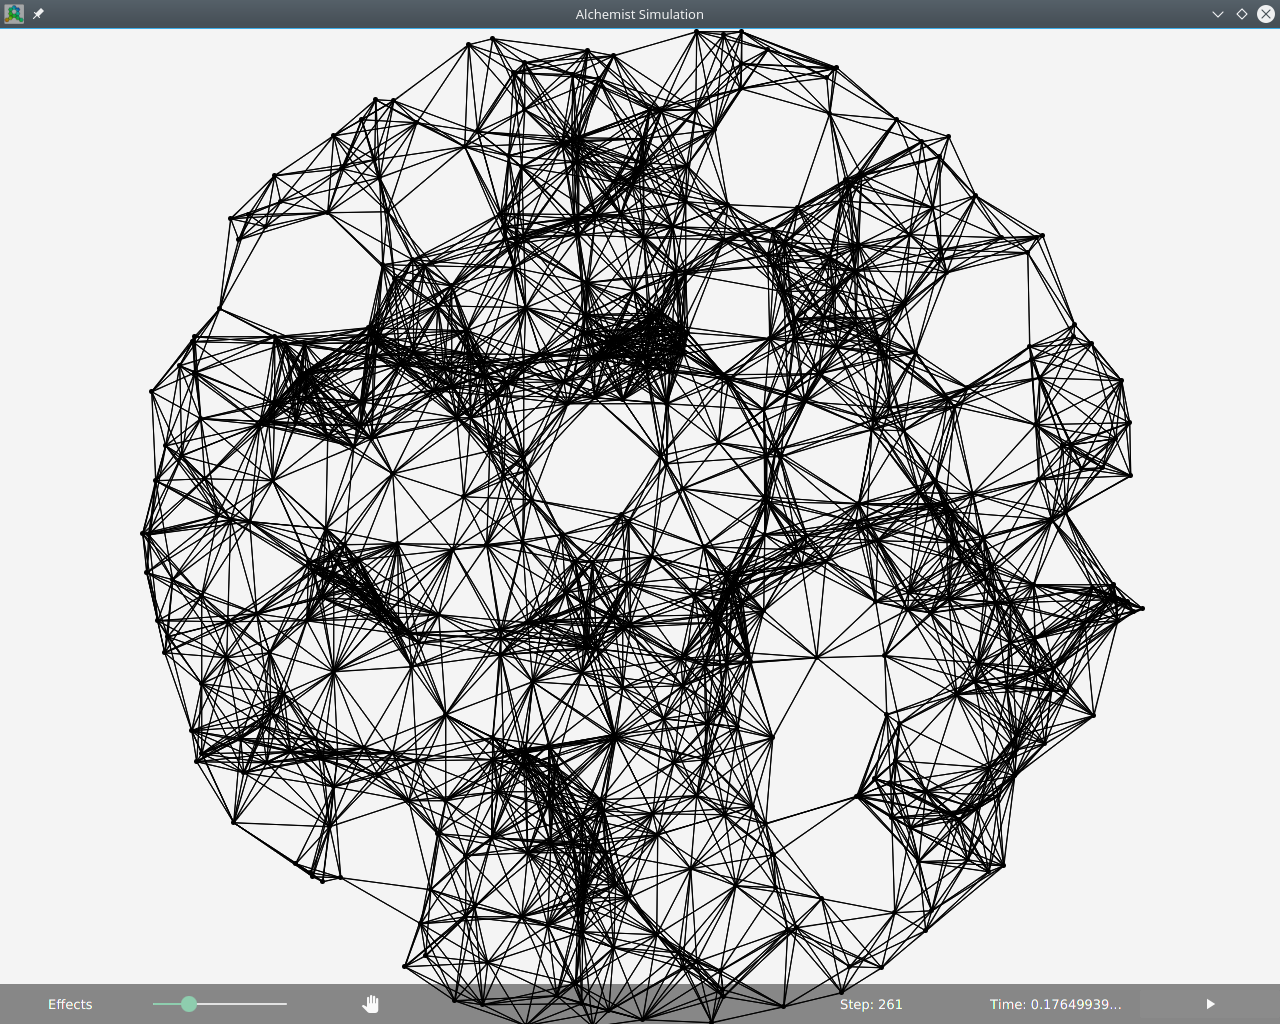
\includegraphics[scale=0.44]{img/withNodes/simWithNodes}
                    \caption{Simulazione in corso di esecuzione}
                    \label{fig:simWithNodes}
                \end{figure}

                A causa della mole di lavoro necessario, non è stato possibile implementare la rappresentazione di ambienti con mappe di sfondo.
